\documentclass[a4paper, 12pt]{article}

\usepackage{ragged2e}

% Set margins
\usepackage[hmargin=2cm, vmargin=2cm]{geometry}

\frenchspacing

% Language packages
\usepackage[utf8]{inputenc}
\usepackage[T1]{fontenc}
\usepackage[magyar]{babel}


% AMS
\usepackage{amssymb,amsmath}

% Graphic packages
\usepackage{graphicx}

% Colors
\usepackage{color}
\usepackage[usenames,dvipsnames]{xcolor}

% Enumeration
\usepackage{enumitem}

% C code
\usepackage{xcolor}
\usepackage{listings}

% Hyperref
\usepackage{hyperref}

\title{\vskip -30pt Adatbázis rendszerek MSc (GEIAL521M)\\\LARGE{\textbf{MongoDB gyakorlat}}}
\date{\vskip -30pt 2021. április 27.}
\author{}

\begin{document}

\begin{titlepage}

\begin{center}


{\Huge \textbf{\vskip 200pt Jegyzőkönyv}}

\bigskip

{\LARGE Adatbázis rendszerek MSc (GEIAL521M)}

\medskip

{\LARGE 2021. tavasz féléves feladat}

\end{center}

\vskip 350pt

\null\hfill{
\large
\begin{tabular}{ l l }
 Készítette: & \textbf{Nagy Dániel Zoltán} \\ 
 Neptun kód: & \texttt{JJ181J}  
\end{tabular}
}

\end{titlepage}


\maketitle

\section*{1. feladat}
Hozzon létre egy kollekciót, amelyben zenei albumokat tárol.\\
Egy-egy albumot az alábbi tulajdonságokkal jellemezhetünk:
\begin{itemize}[noitemsep]
	\item cím
	\item előadó
	\item ország
	\item megjelenés éve
	\item műfaj
	\item stílus(ok)
	\item ár
\end{itemize}
Esetünkben az \_id lehet globális/gyári is.

\begin{enumerate}[label=\textbf{\alph*)}]
\item Vigyen fel adatokat, amelyekkel a továbbiakban dolgozhat!
\item Az albumokon hajtson végre szűrési feltételeket:
	  \begin{itemize}[label=-]
	  \item Kérje le az 1971-nél frissebb albumok címeit és megjelenési éveit!
	  \item Kérje le a 21\$-nál olcsóbb angol albumok címeit és árait!
	  \item Kérje le a legolcsóbb album adatait!
	  \end{itemize}
\item Hajtson végre módosító műveleteket az alábbiak szerint:
	  \begin{itemize}[label=-]
	  \item Módosítsa egy tetszőleges album címét!
	  \item Egy tetszőleges album stílusai közé vigyen fel egy új stílust!
	  \item Egy akció keretében a 70-es évekbeli Rock műfajú albumok árai 20$\%$-al csökkennek.\\Végezze el a szükséges módosításokat!
	  \item Adjon mindegyik albumhoz egy új mezőt, és írjon be mindegyikbe egy-egy random számot!
	  \end{itemize}
\end{enumerate}
\newpage
\subsection*{Megoldás}
Első lépésként \textit{Tunellezéssel} érjük el a tanszéki MongoDB szervert. Ezt megtehetjük \textit{MobaXterm} ssh kliens segítségével is, vagy Linux Mint esetén a gyári ssh-val a következő módon:
\begin{figure}[!hb]
	\centering
	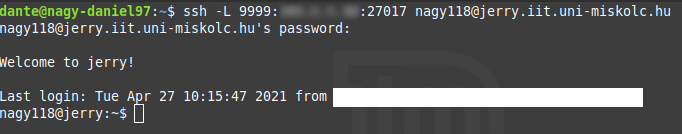
\includegraphics[scale = 0.7]{images/0_tunelling.png}
	\label{fig:0_tunelling}
\end{figure}

\noindent Ha sikerült csatlakoznunk, a megadott porton keresztül érhetjük el a szervert.\\
A megoldások során a \textit{Robo3T} klienssel kezeljük az adatbázist.\\
Új kapcsolat felvételénél a következőket kell megadnunk:
\begin{figure}[!hb]
	\centering
	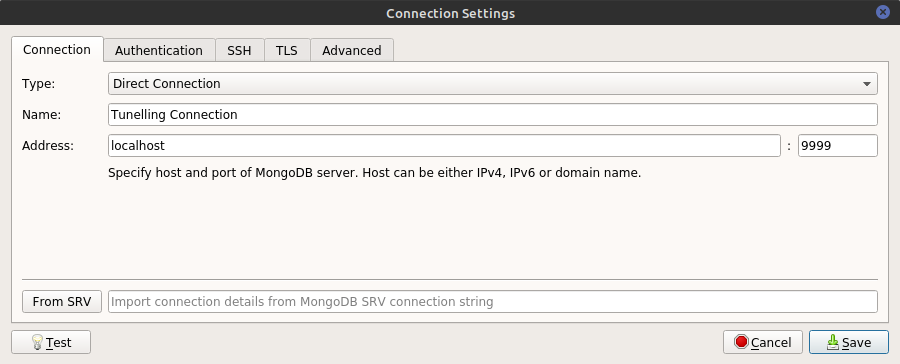
\includegraphics[scale = 0.5]{images/0_Robo_connect.png}
	\label{fig:0_Robo_connect}
\end{figure}	

\subsubsection*{a)}
Nyisson egy új shellt!\\
A \texttt{use} paranccsal tudunk új adatbázist létrehozni.
\begin{figure}[!hb]
	\centering
	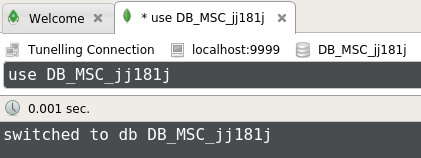
\includegraphics[scale = 0.7]{images/0_useDB.png}
	\label{fig:0_useDB}
\end{figure}

\noindent Vigyen fel adatokat, amelyekkel a továbbiakban dolgozhat!
\clearpage
\begin{figure}[!hb]
	\centering
	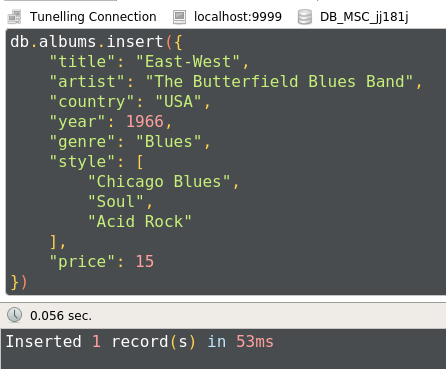
\includegraphics[scale = 0.45]{images/1_a1.png}
	\label{fig:1_a1}
\end{figure}	

\begin{tabular}{ c c }
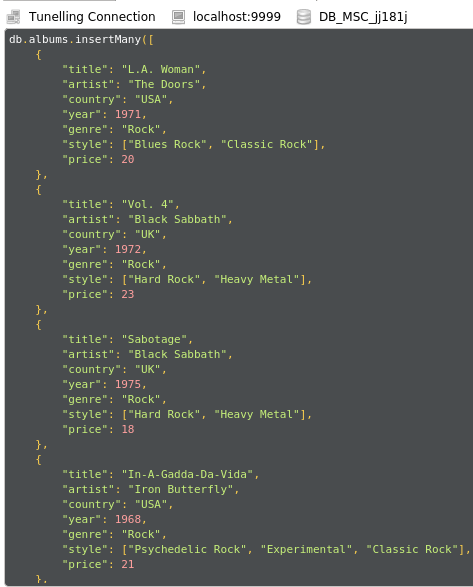
\includegraphics[scale = 0.45]{images/1_a2.png} & 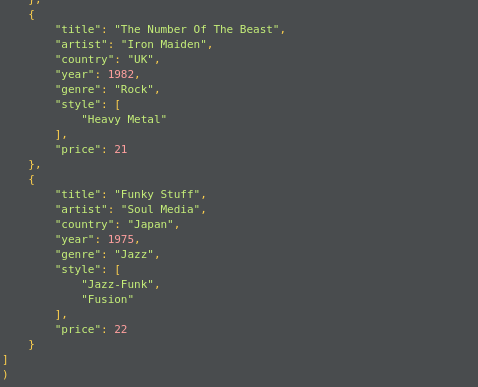
\includegraphics[scale = 0.45]{images/1_a3.png}
\end{tabular}

\begin{figure}[!hb]
	\centering
	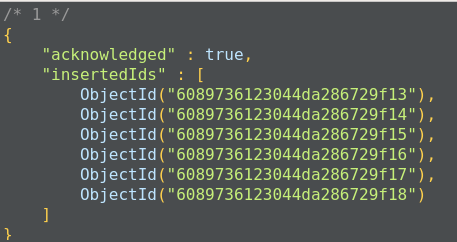
\includegraphics[scale = 0.4]{images/1_a4.png}
	\label{fig:1_a4}
\end{figure}	

\begin{figure}[!hb]
	\centering
	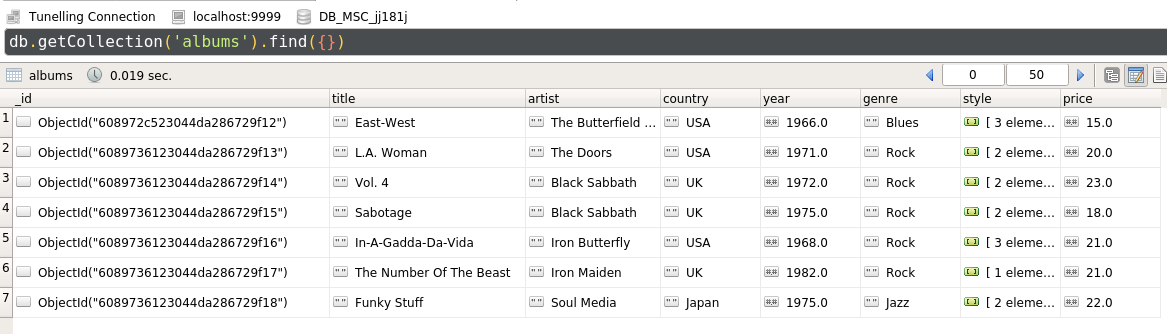
\includegraphics[scale = 0.4]{images/1_a5.png}
	\label{fig:1_a5}
\end{figure}
\clearpage
\subsubsection*{b)}
Kérje le az 1971-nél frissebb albumok címeit és megjelenési éveit!
\begin{figure}[!hb]
	\centering
	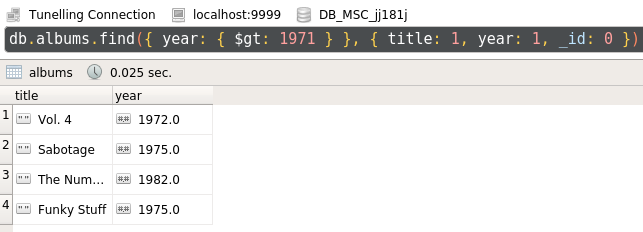
\includegraphics[scale = 0.55]{images/1_b1.png}
	\label{fig:1_b1}
\end{figure}

\noindent Kérje le a 21\$-nál olcsóbb angol albumok címeit és árait!
\begin{figure}[!hb]
	\centering
	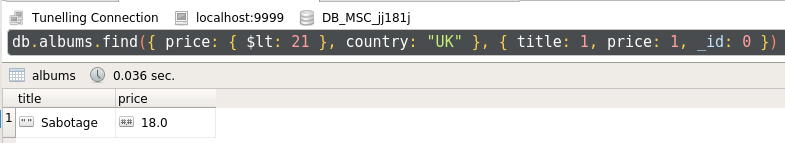
\includegraphics[scale = 0.55]{images/1_b2.png}
	\label{fig:1_b2}
\end{figure}

\noindent Egy másik megoldás a \texttt{\$where} operátorral:
\begin{figure}[!hb]
	\centering
	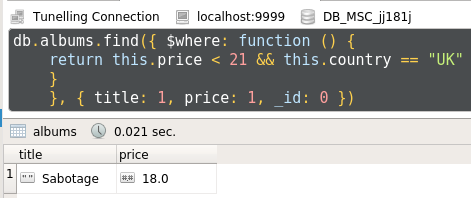
\includegraphics[scale = 0.55]{images/1_b3.png}
	\label{fig:1_b3}
\end{figure}

\noindent Kérje le a legolcsóbb album adatait!
\begin{figure}[!hb]
	\centering
	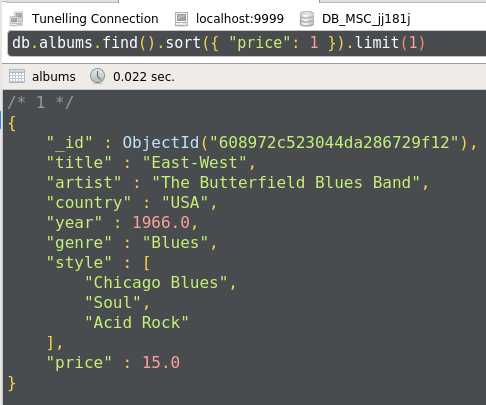
\includegraphics[scale = 0.55]{images/1_b4.png}
	\label{fig:1_b4}
\end{figure}	
\clearpage
\subsubsection*{c)}
\noindent Módosítsa egy tetszőleges album címét!
\begin{figure}[!hb]
	\centering
	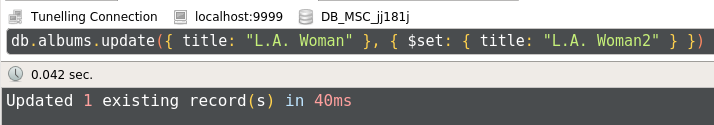
\includegraphics[scale = 0.6]{images/1_c1.png}
	\label{fig:1_c1}
\end{figure}	

\noindent Egy tetszőleges album stílusai közé vigyen fel egy új stílust!
\begin{figure}[!hb]
	\centering
	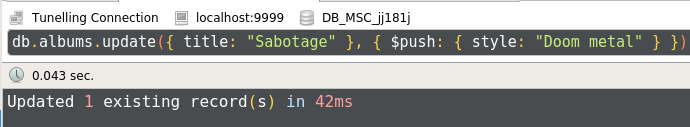
\includegraphics[scale = 0.6]{images/1_c2.png}
	\label{fig:1_c2}
\end{figure}	

\noindent Egy akció keretében a 70-es évekbeli Rock műfajú albumok árai 20$\%$-al csökkennek.\\Végezze el a szükséges módosításokat!
\begin{figure}[!hb]
	\centering
	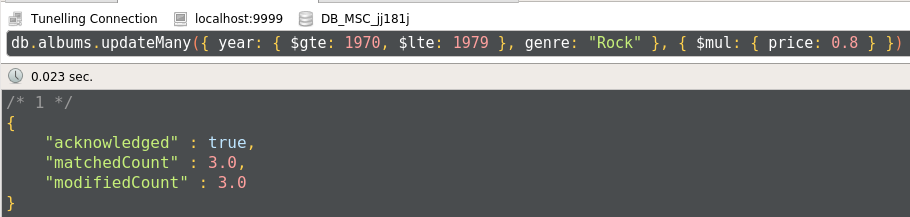
\includegraphics[scale = 0.5]{images/1_c3.png}
	\label{fig:1_c3}
\end{figure}	

\noindent Adjon mindegyik albumhoz egy új mezőt, és írjon be mindegyikbe egy-egy random számot!
\begin{figure}[!hb]
	\centering
	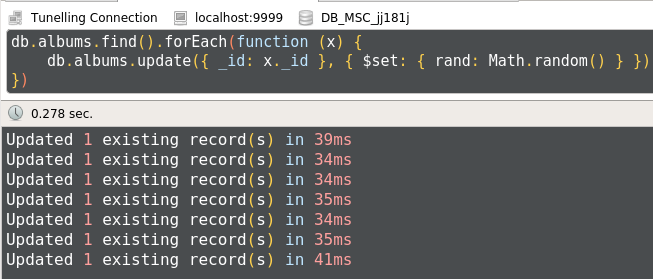
\includegraphics[scale = 0.6]{images/1_c4.png}
	\label{fig:1_c4}
\end{figure}	
\clearpage

\section*{2. feladat}
Hozzon létre egy új kollekciót, amelyben az előadók adatait tárolja.\\
Az egyes előadókat a következő tulajdonságok jellemzik:
\begin{itemize}[noitemsep]
	\item név
	\item ország
\end{itemize}
\begin{enumerate}[label=\textbf{\alph*)}]
\item Vigye fel az 1. feladatban feltöltött albumok előadóinak az adatait!
\item Írjon egy olyan szerveroldali függvényt, amely elvégzi a következő módosításokat az albumok kollekcióján:
	  \begin{itemize}[label=-]
	  \item az előadó neve helyére az albumhoz tartozó előadó \_id-jét redeli.
	  \item az ország mezőket törli, hiszen az előadó adatai között már szerepelnek.
	  \end{itemize}
\item Írjon egy olyan szerveroldali függvényt, amely segítségével egy kiválaszott műfaj százalékos árcsökkentését elvégezhetjük.\\Az eredményt egy új kollekcióba mentse, ne írja felül az eredeti adatokat!
\item Írjon egy olyan függvényt, amely lekérdezi az átlagárnál drágább albumok címeit!
\item Hajtson végre aggregációs műveleteket
	  \begin{itemize}[label=-]
	  \item Számítsa ki az egyes műfajokhoz tartozó átlagárat forintban (1 USD 300 magyar forintnak felel meg)!
	  \item Számolja meg, hogy az egyes műfajokban hány 20\$-nál drágább album van és az eredményt rendezze darabszám szerinti csökkenő sorrendben!
	  \item Kérdezze le a legolcsóbb albumot az előadó adataival kiegészítve!
	  \item Keresse meg, hogy mely előadóhoz tartozik a legtöbb album, majd írassa ki az előadó nevét és a hozzá tartozó album címek listáját, valamint a legolcsóbb lemezének az árát!
	  \end{itemize}
\end{enumerate}
\newpage
\subsection*{Megoldás}

\subsubsection*{a)}
Vigye fel az 1. feladatban feltöltött albumok előadóinak az adatait!
\begin{figure}[!hb]
	\centering
	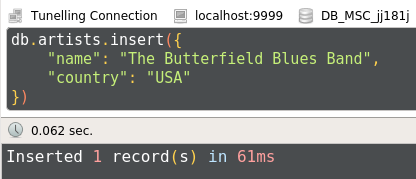
\includegraphics[scale = 0.65]{images/2_a1.png}
	\label{fig:2_a1}
\end{figure}
\begin{figure}[!hb]
	\centering
	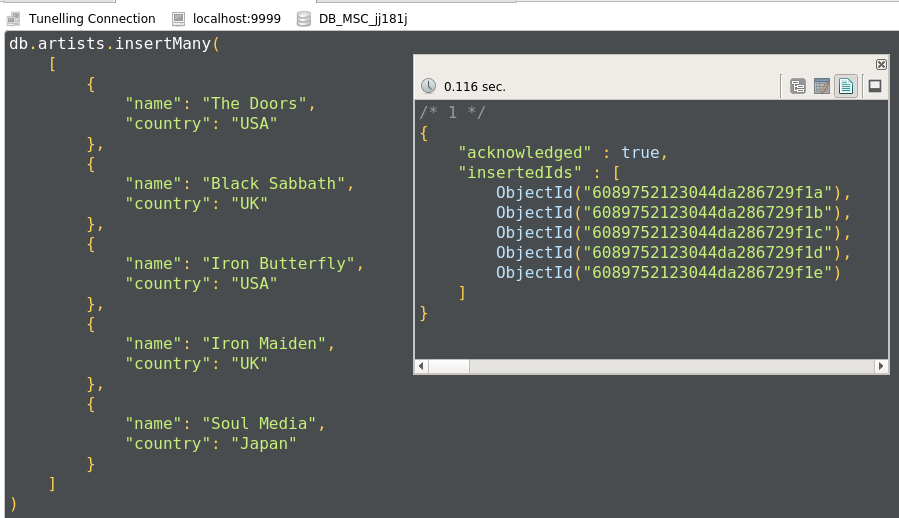
\includegraphics[scale = 0.5]{images/2_a2.png}
	\label{fig:2_a2}
\end{figure}
\clearpage
\subsubsection*{b)}
Írjon egy olyan szerveroldali függvényt, amely elvégzi a következő módosításokat az albumok kollekcióján:
\begin{itemize}[label=-]
\item az előadó neve helyére az albumhoz tartozó előadó \_id-jét redeli.
\item az ország mezőket törli, hiszen az előadó adatai között már szerepelnek.
\end{itemize}
\begin{figure}[!hb]
	\centering
	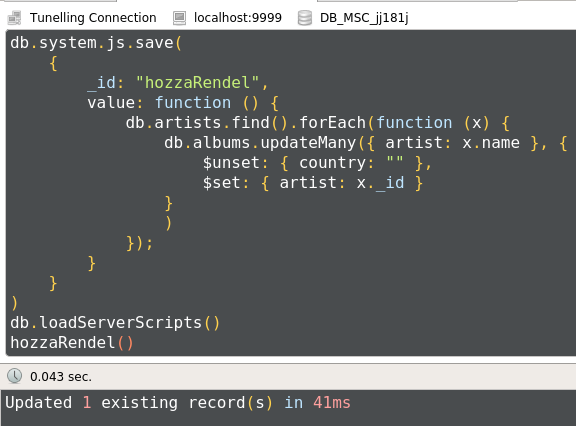
\includegraphics[scale = 0.65]{images/2_b1.png}
	\label{fig:2_b1}
\end{figure}
\begin{figure}[!hb]
	\centering
	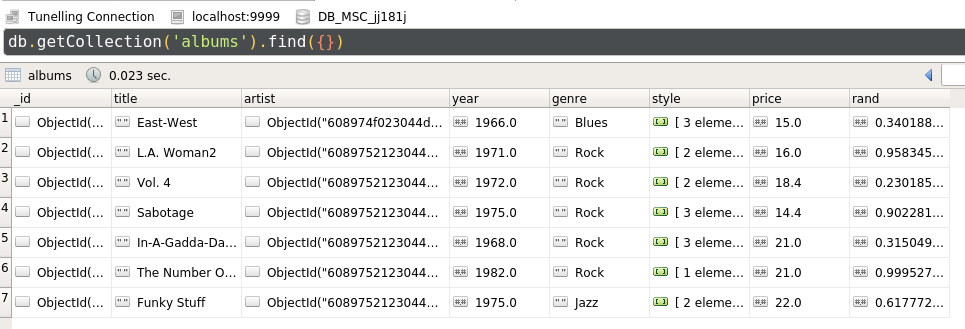
\includegraphics[scale = 0.45]{images/2_b2.png}
	\label{fig:2_b2}
\end{figure}
\clearpage
\subsubsection*{c)}
Írjon egy olyan szerveroldali függvényt, amely segítségével egy kiválaszott műfaj százalékos árcsökkentését elvégezhetjük.\\Az eredményt egy új kollekcióba mentse, ne írja felül az eredeti adatokat!
\begin{figure}[!hb]
	\centering
	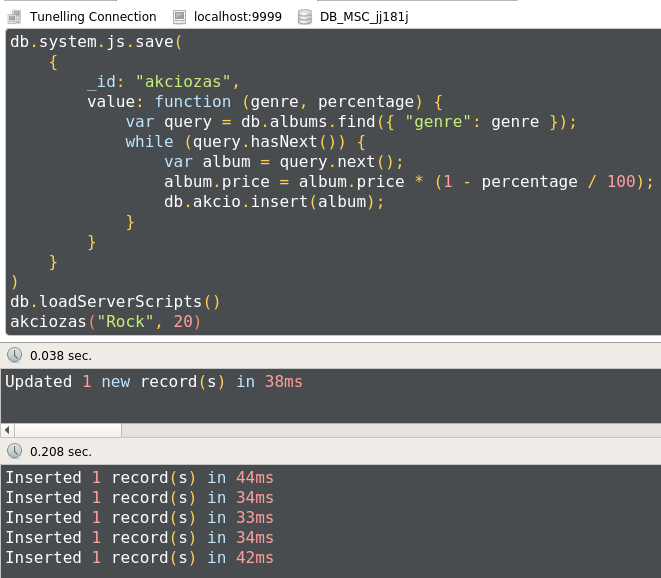
\includegraphics[scale = 0.65]{images/2_c1.png}
	\label{fig:2_c1}
\end{figure}
\begin{figure}[!hb]
	\centering
	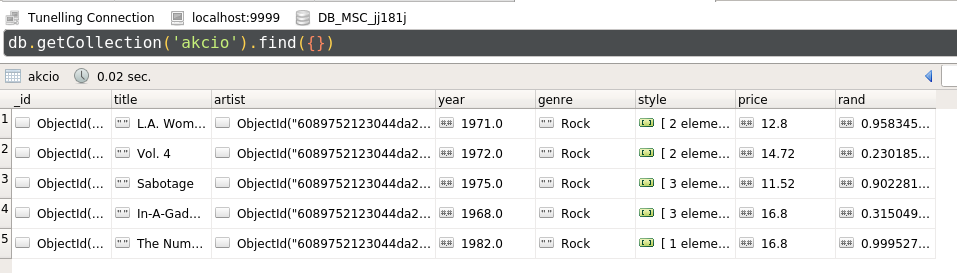
\includegraphics[scale = 0.45]{images/2_c2.png}
	\label{fig:2_c2}
\end{figure}
\clearpage
\subsubsection*{d)}
Írjon egy olyan függvényt, amely lekérdezi az átlagárnál drágább albumok címeit!
\begin{figure}[!hb]
	\centering
	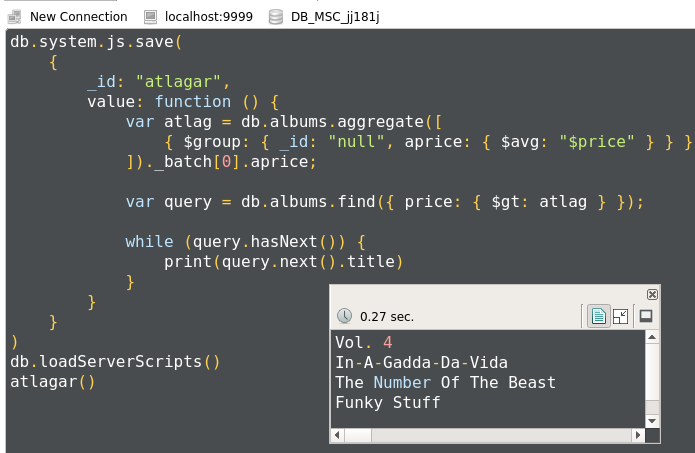
\includegraphics[scale = 0.65]{images/2_d1.png}
	\label{fig:2_d1}
\end{figure}
\clearpage
\subsubsection*{e)}
Számítsa ki az egyes műfajokhoz tartozó átlagárat forintban (1 USD 300 magyar forintnak felel meg)!
\begin{figure}[!hb]
	\centering
	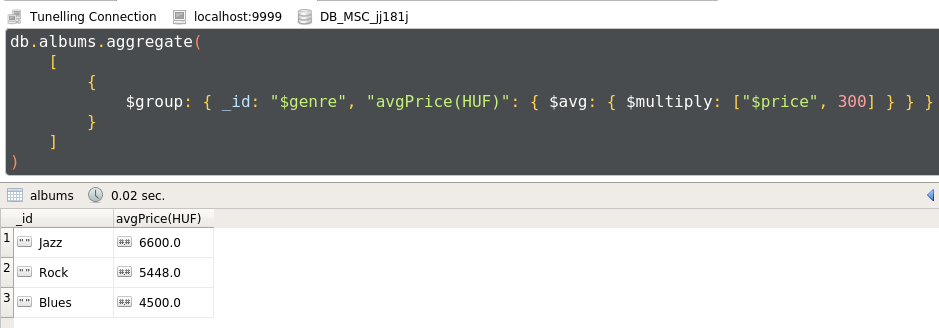
\includegraphics[scale = 0.5]{images/2_e1.png}
	\label{fig:2_e1}
\end{figure}

\noindent Számolja meg, hogy az egyes műfajokban hány 20\$-nál drágább album van és az eredményt rendezze darabszám szerinti csökkenő sorrendben!
\begin{figure}[!hb]
	\centering
	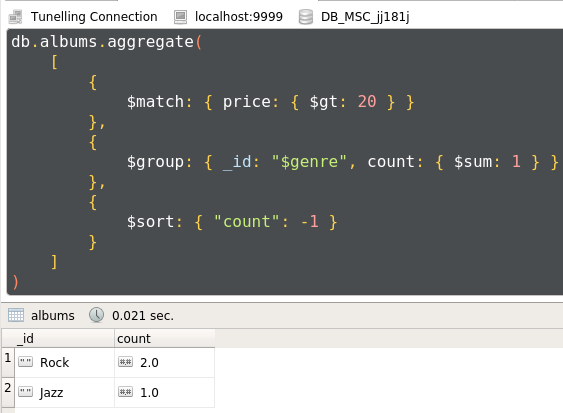
\includegraphics[scale = 0.6]{images/2_e2.png}
	\label{fig:2_e2}
\end{figure}
\newpage
\noindent Kérdezze le a legolcsóbb albumot az előadó adataival kiegészítve!
\begin{figure}[!hb]
	\centering
	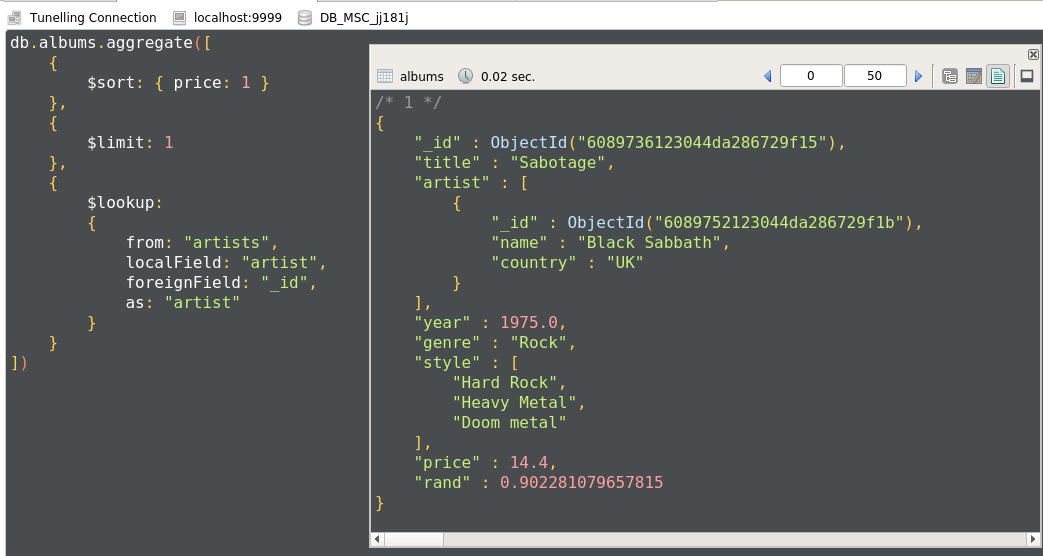
\includegraphics[scale = 0.46]{images/2_e3.png}
	\label{fig:2_e3}
\end{figure}

\noindent Keresse meg, hogy mely előadóhoz tartozik a legtöbb album, majd írassa ki az előadó nevét és a hozzá tartozó album címek listáját, valamint a legolcsóbb lemezének az árát!
\begin{figure}[!hb]
	\centering
	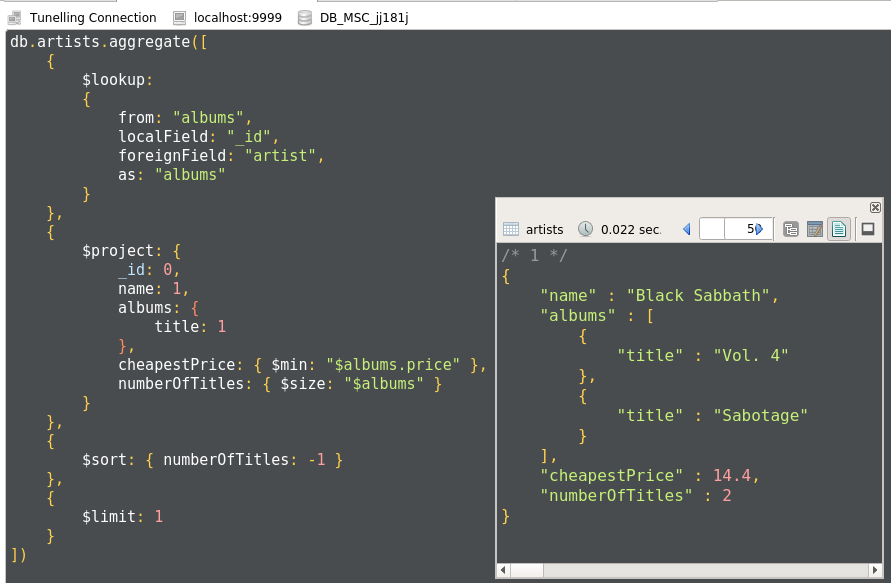
\includegraphics[scale = 0.53]{images/2_e4.png}
	\label{fig:2_e4}
\end{figure}	
\clearpage

\section*{3. feladat}
Írjon egy Python nyelvű programot, amely az alapvető CRUD(Create Read Update Delete) műveleteket tudja eszközölni a fentiekben létrehozott adatbázison!\\
Néhány javasolt funkció:
\begin{enumerate}
	\item Albumok kilistázása
	\item Előadók kilistázása
	\item Új előadó felvitele
	\item Album címének módosítása
	\item Album törlése cím alapján
\end{enumerate}
Létesítsen kapcsolatot az adatbázissal és valósítsa meg a felsorolt funkciókat!\\
A megoldás során javasolt a \texttt{PyMongo} használata.
\newpage
\subsection*{Megoldás}
{\large Forráskód:}
\begin{figure}[!hb]
	\centering
	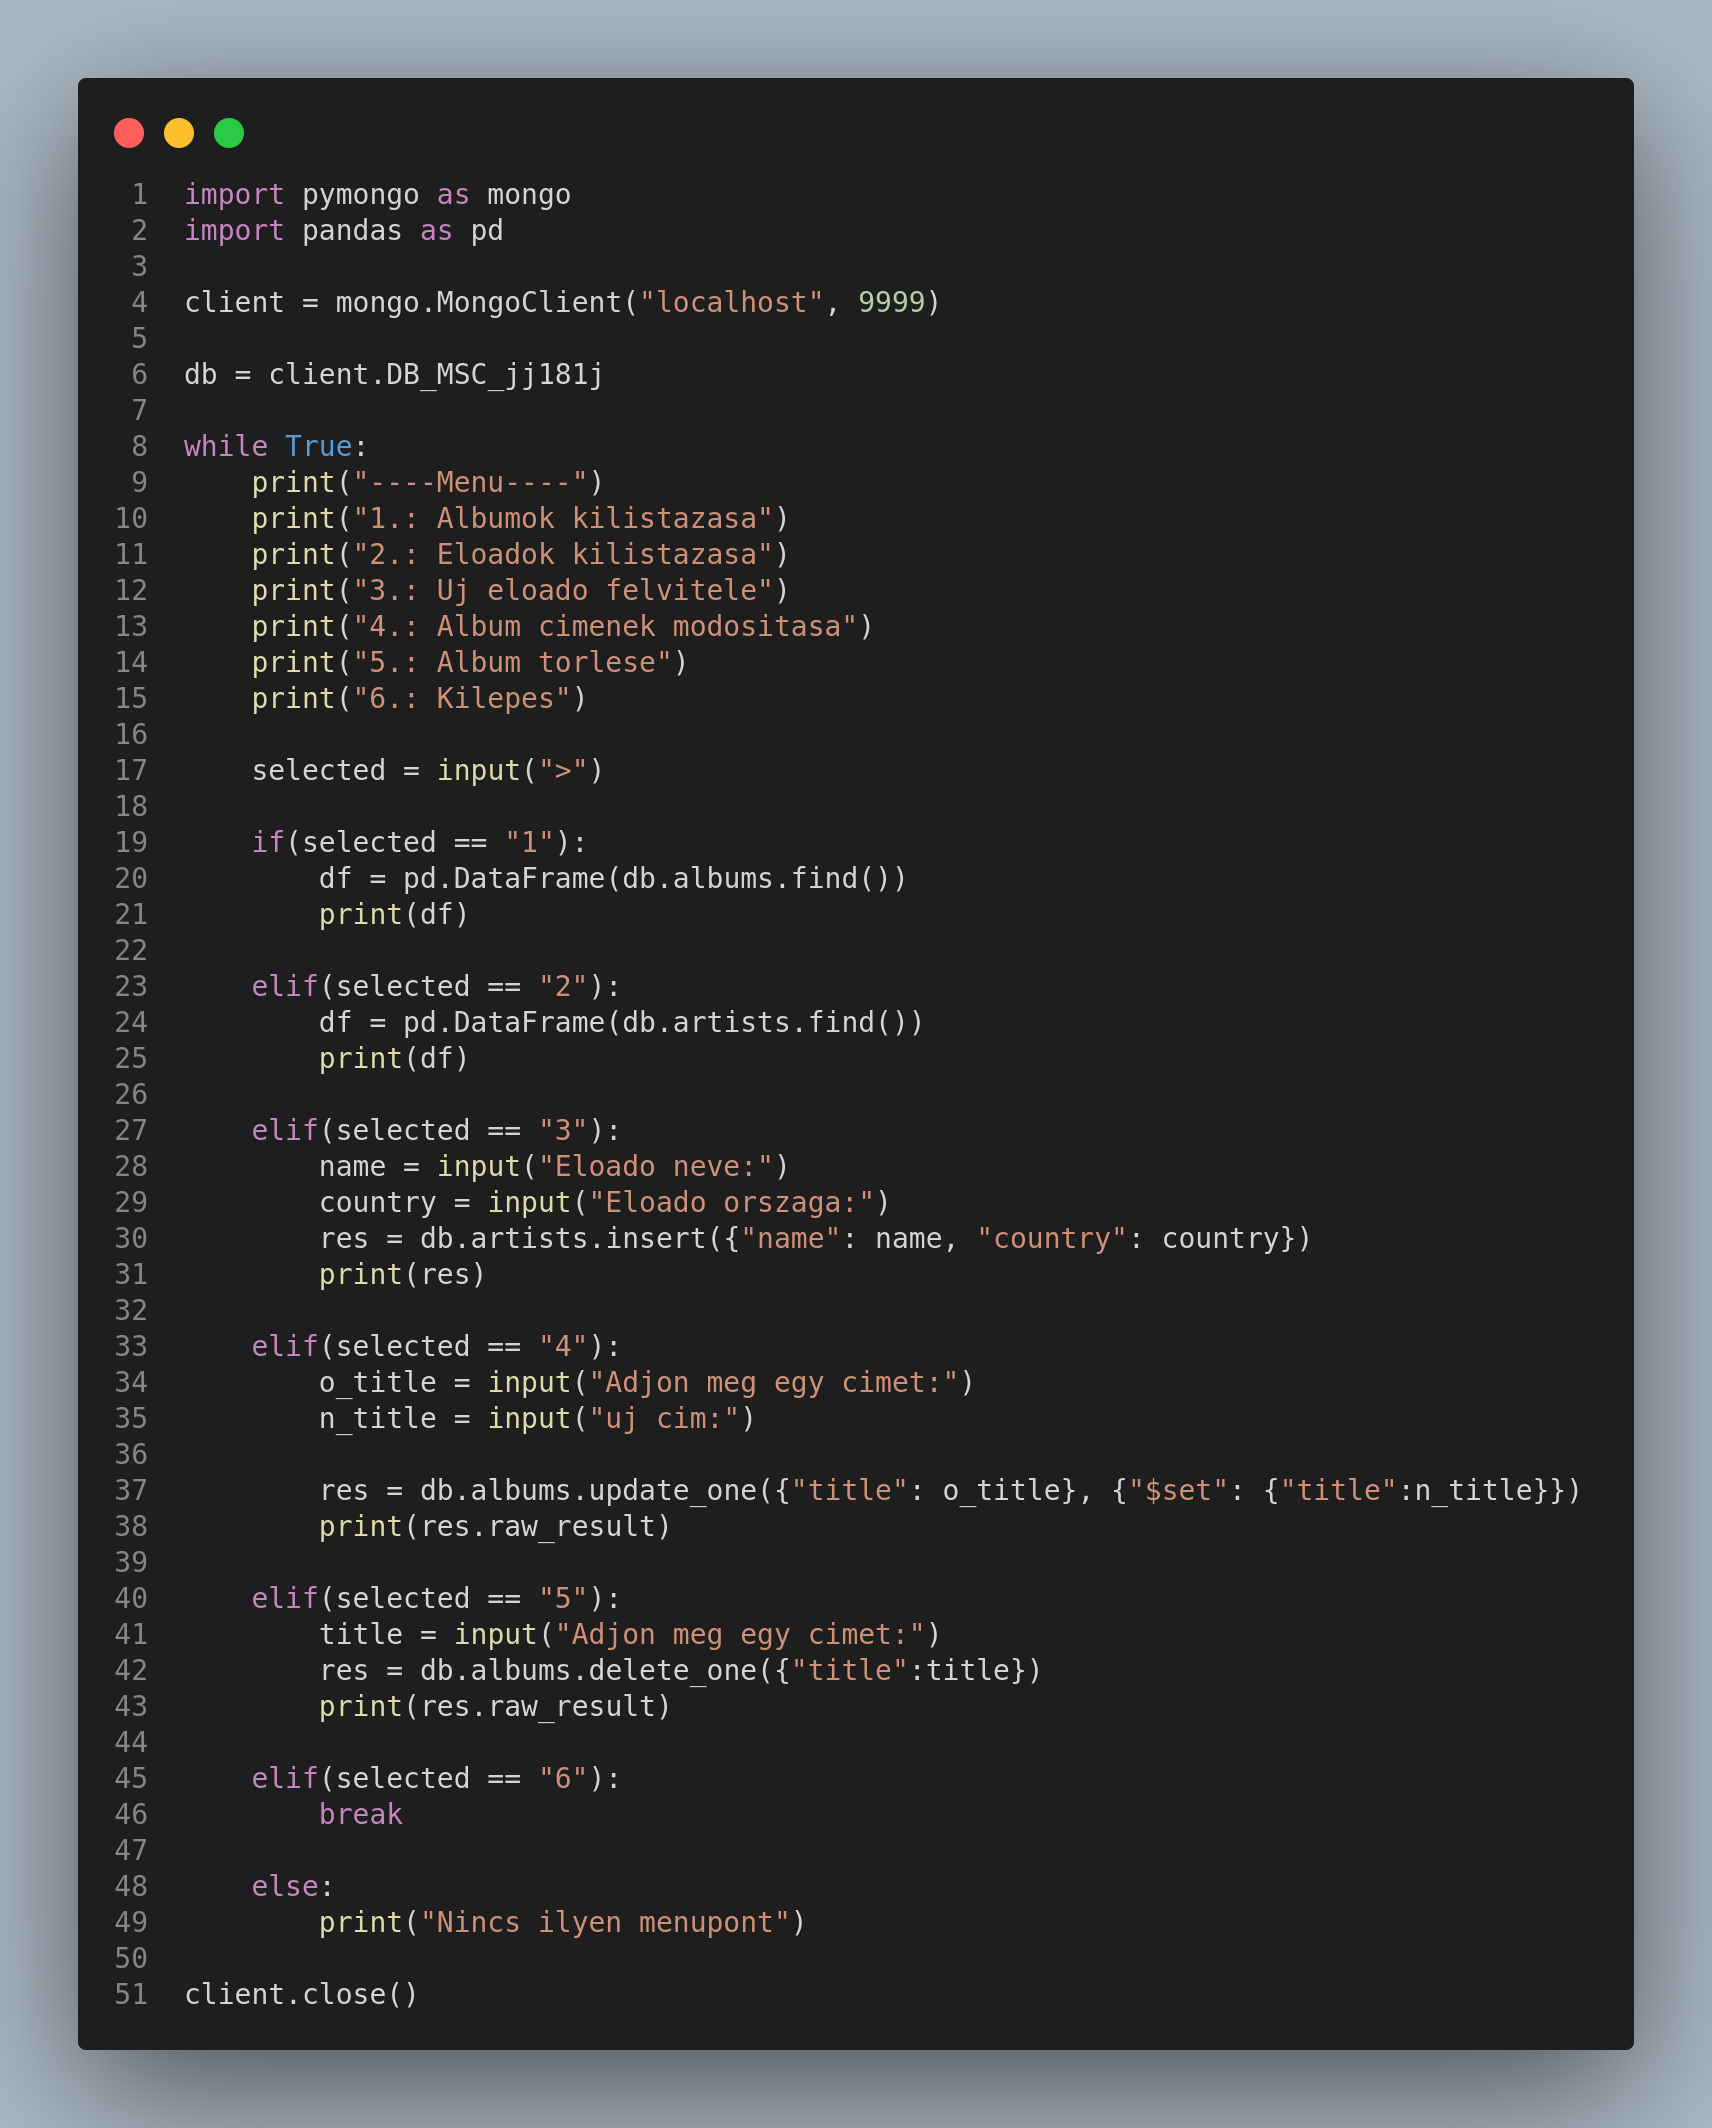
\includegraphics[width = 17cm]{images/3_code.png}
	\label{fig:3_code}
\end{figure}	
\newpage
{\large Futási eredmények:}
\begin{figure}[!hb]
	\centering
	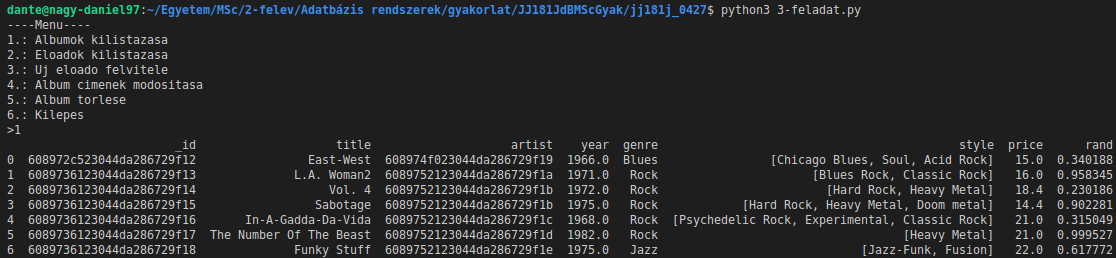
\includegraphics[scale = 0.4]{images/3_out1.png}
	\label{fig:3_out1}
\end{figure}
\begin{figure}[!hb]
	\centering
	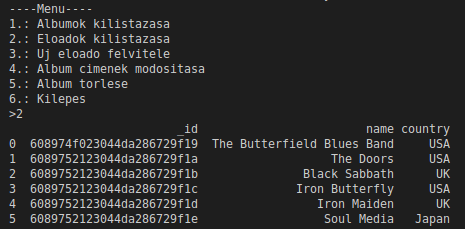
\includegraphics[scale = 0.7]{images/3_out2.png}
	\label{fig:3_out2}
\end{figure}	
\begin{figure}[!hb]
	\centering
	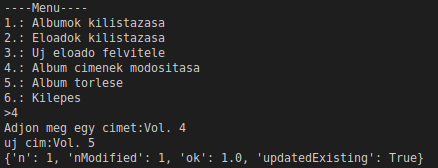
\includegraphics[scale = 0.7]{images/3_out4.png}
	\label{fig:3_out4}
\end{figure}	

\bigskip

\begin{tabular}{ c c }
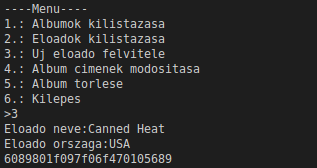
\includegraphics[scale = 0.7]{images/3_out3.png} & 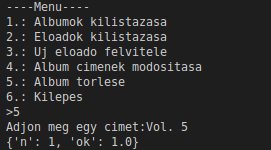
\includegraphics[scale = 0.7]{images/3_out5.png}
\end{tabular}

\end{document}
